\documentclass[a4paper]{article}
\usepackage[utf8]{inputenc}\usepackage[T1]{fontenc}\usepackage{helvet}\renewcommand{\familydefault}{\sfdefault}
\usepackage[a4paper,margin=2.2cm]{geometry}\usepackage{graphicx}\usepackage{xcolor}\usepackage{pdfpages}\usepackage[hidelinks]{hyperref}\usepackage{tabularx}\usepackage{colortbl}
\definecolor{uteqverde}{HTML}{2C5F2D}\definecolor{uteqazul}{HTML}{1E4D8B}\definecolor{grisclaro}{HTML}{F2F2F2}\setlength{\parindent}{0pt}
\newcommand{\notaprov}{3{,}37}\newcommand{\completitud}{64\,\%}
\let\notaFUVV\notaprov\let\compFUVV\completitud\let\notaprov\relax\let\completitud\relax
\newcommand{\notaprov}{2{,}64}\newcommand{\completitud}{55\,\%}
\let\notaACC\notaprov\let\compACC\completitud\let\notaprov\relax\let\completitud\relax
\newcommand{\notaprov}{2{,}45}\newcommand{\completitud}{56\,\%}
\let\notaAGLS\notaprov\let\compAGLS\completitud\let\notaprov\relax\let\completitud\relax
\newcommand{\notaprov}{2{,}65}\newcommand{\completitud}{40\,\%}
\let\notaBCEL\notaprov\let\compBCEL\completitud
\begin{document}
\begin{center}
\includegraphics[width=\textwidth]{logoband.png}\\[24pt]
{\LARGE\bfseries\color{uteqverde} Gu\'ias de cierre y r\'ubricas del examen suspenso}\\[6pt]
{\Large\bfseries\color{uteqazul} Proyecto Fin de Curso --- Aplicaciones Distribuidas (ISR-701)}\\[14pt]
{\large Universidad T\'ecnica Estatal de Quevedo \textperiodcentered{} 2026--2027 PPA \textperiodcentered{} S\'eptimo semestre ``A'' Software}\\[6pt]
{\large Estado evaluado: domingo 13 de septiembre de 2026, 19:00 \textperiodcentered{} Corte: viernes 18 de septiembre de 2026, 23:55}\\[24pt]\end{center}
{\large\bfseries\color{uteqverde} Contenido y estado al 13/09/2026, 19:00}\\[6pt]
{\small\begin{tabularx}{\textwidth}{|p{1.4cm}|X|p{4.0cm}|p{1.9cm}|p{2.0cm}|}\hline
\rowcolor{uteqverde}\textcolor{white}{\bfseries Equipo}&\textcolor{white}{\bfseries Sistema}&\textcolor{white}{\bfseries Repositorio}&\textcolor{white}{\bfseries Completitud}&\textcolor{white}{\bfseries Nota provisional}\\ \hline
\hyperlink{fuvv}{FUVV} & SCLI, Sistema de Control de Laboratorios Inform\'aticos & \texttt{\footnotesize gleiston-guerrero/\allowbreak Entrega-final-del-PFC} & \compFUVV & \notaFUVV{} / 10 \\ \hline
\hyperlink{acc}{ACC} & TicketFold, soporte t\'ecnico distribuido para un proveedor de Internet & \texttt{\footnotesize gleiston-guerrero/\allowbreak PFC-SOPORTE-ISP} & \compACC & \notaACC{} / 10 \\ \hline
\hyperlink{agls}{AGLS} & TiendaTech, comercio electr\'onico distribuido (repositorio \textbf{sin transferir}) & \texttt{\footnotesize JoseLozanoMorales/\allowbreak TiendaTech} & \compAGLS & \notaAGLS{} / 10 \\ \hline
\hyperlink{bcel}{BCEL} & AcadTrace, gesti\'on acad\'emica con bit\'acora de auditor\'ia encadenada & \texttt{\footnotesize gleiston-guerrero/\allowbreak acadtrace} & \compBCEL & \notaBCEL{} / 10 \\ \hline
\end{tabularx}}\par
\vspace{10pt}{\footnotesize La completitud es el promedio del estado efectivo de los veinte entregables exigidos por la gu\'ia de la Entrega 4, con la regla de dependencia. La nota provisional es la de la r\'ubrica del examen suspenso con el estado encontrado en el \'ultimo commit anterior al 13/09/2026 a las 19:00: s\'olo punt\'uan los \'items que no estaban en Hecho, con pesos proporcionales a profundidad, complejidad, amplitud y tiempo de dedicaci\'on, y coeficientes Hecho 1,00 \textperiodcentered{} Por modificar 0,40 \textperiodcentered{} Por culminar 0,20 \textperiodcentered{} Por iniciar 0,00. Cl\'ausulas comunes: repositorio transferido y aceptado por el docente al corte (en caso contrario, examen no entregado) y car\'atula de una sola p\'agina subida al SGA por cada estudiante. Ing. Gleiston Cicer\'on Guerrero Ulloa, PhD.}
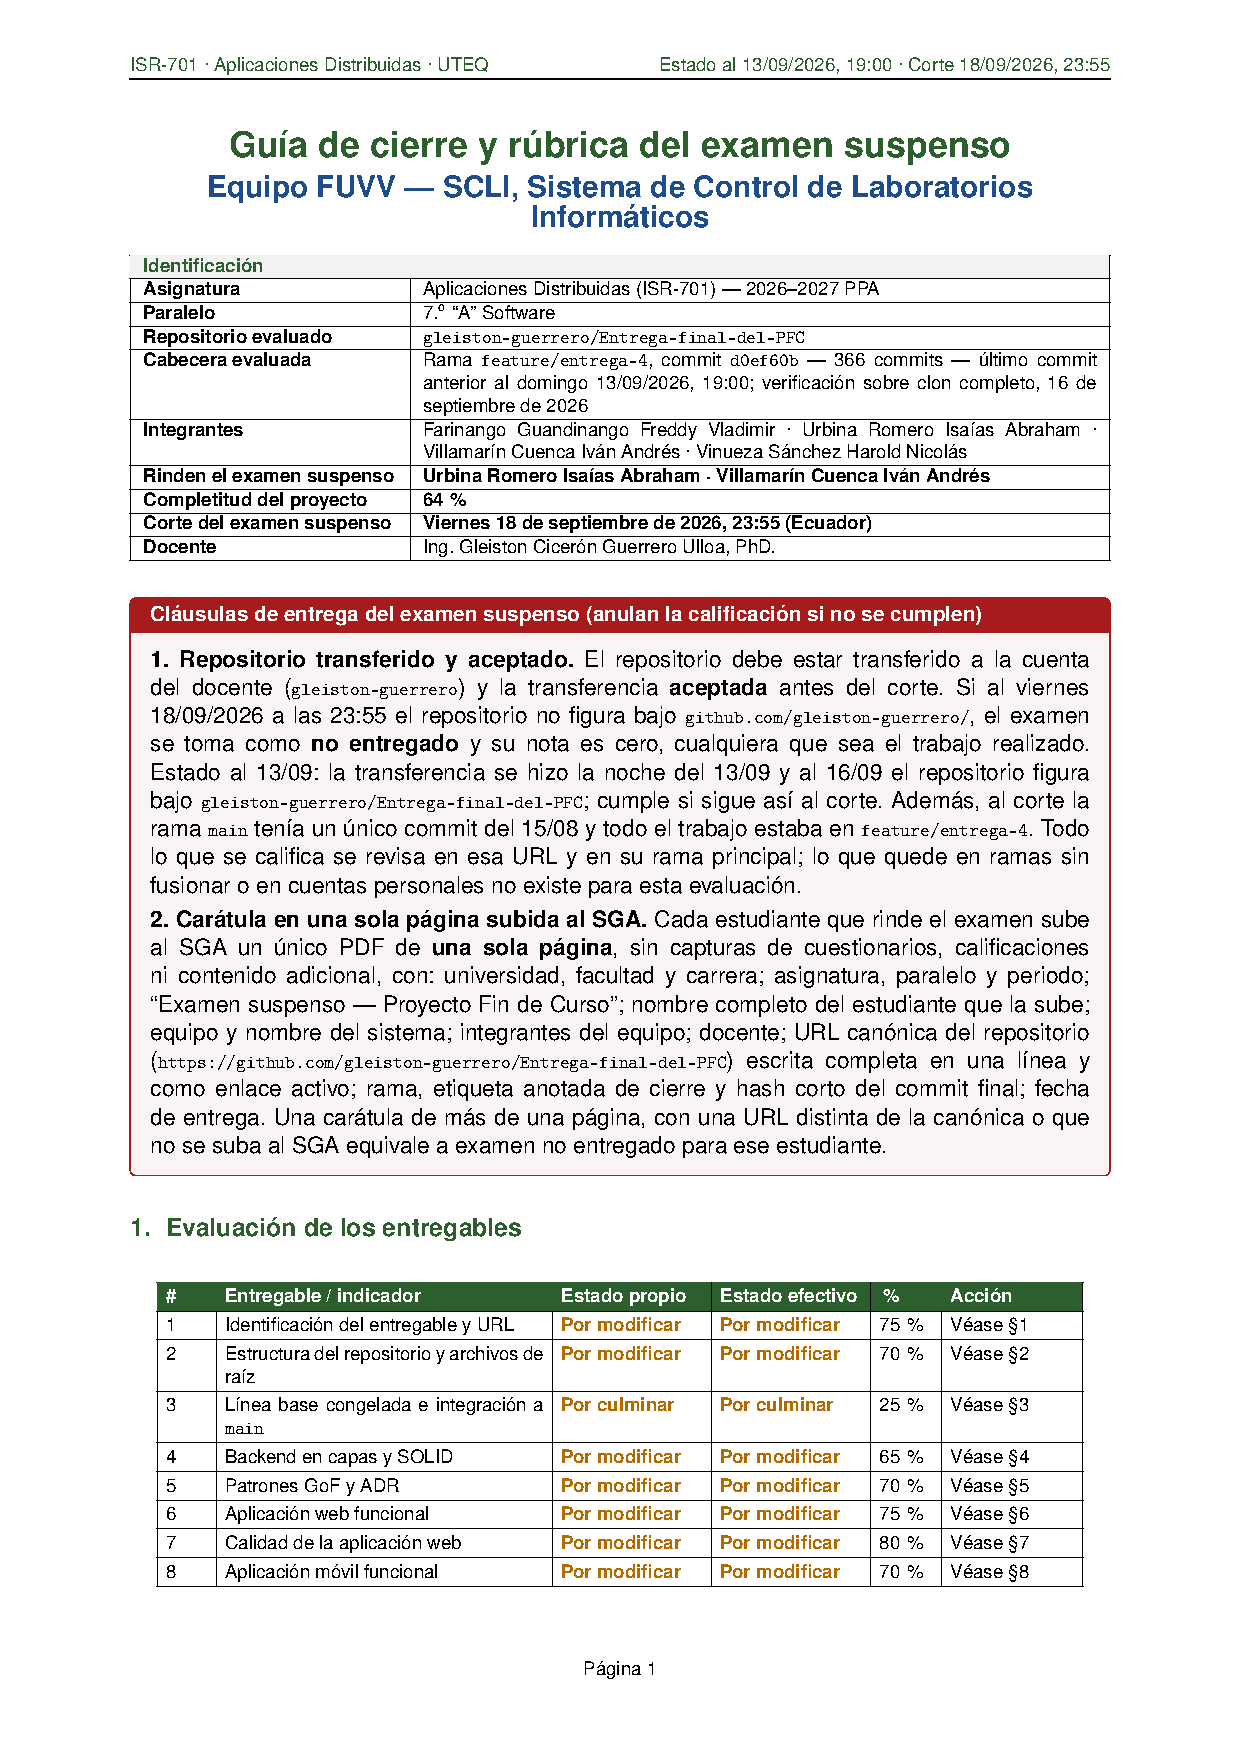
\includepdf[pages=-,addtotoc={1,section,1,FUVV,fuvv}]{Guia_FUVV.pdf}
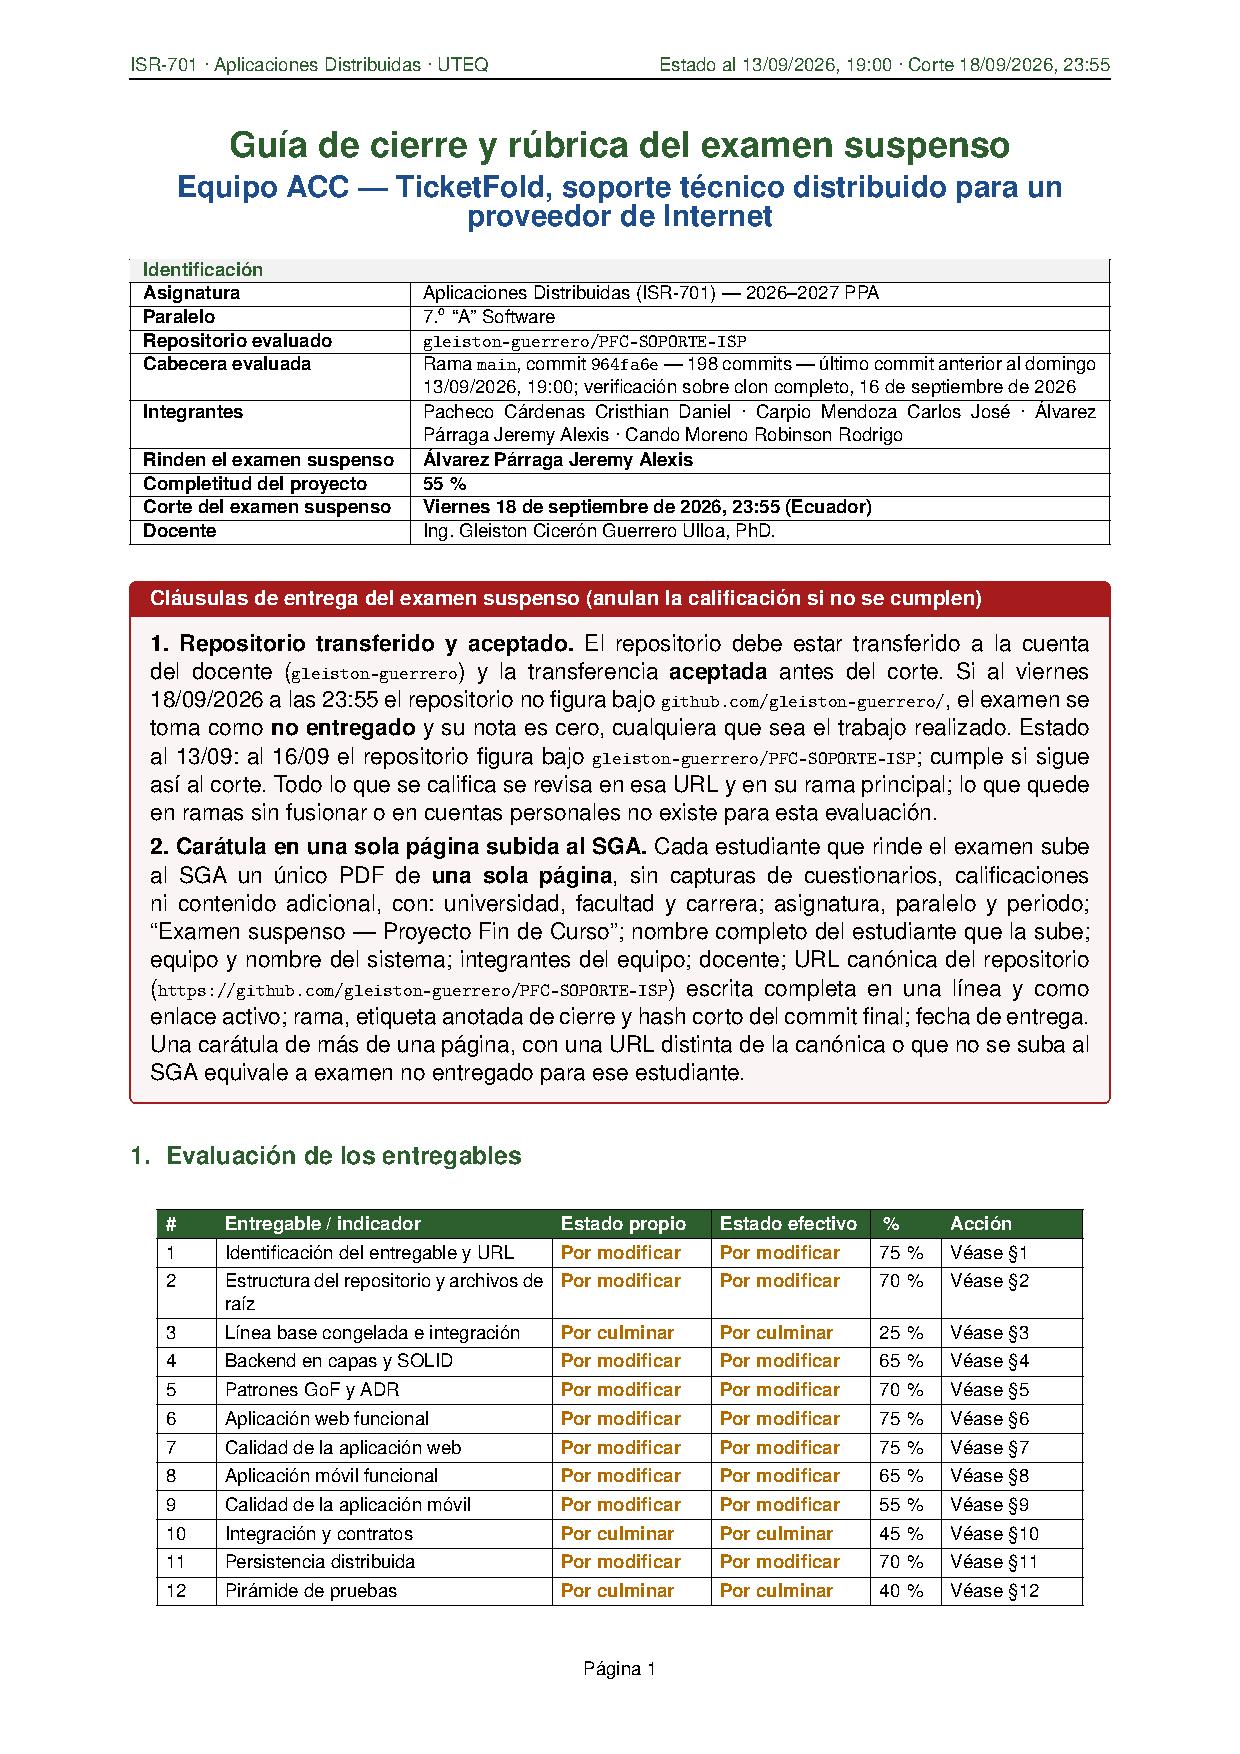
\includepdf[pages=-,addtotoc={1,section,1,ACC,acc}]{Guia_ACC.pdf}
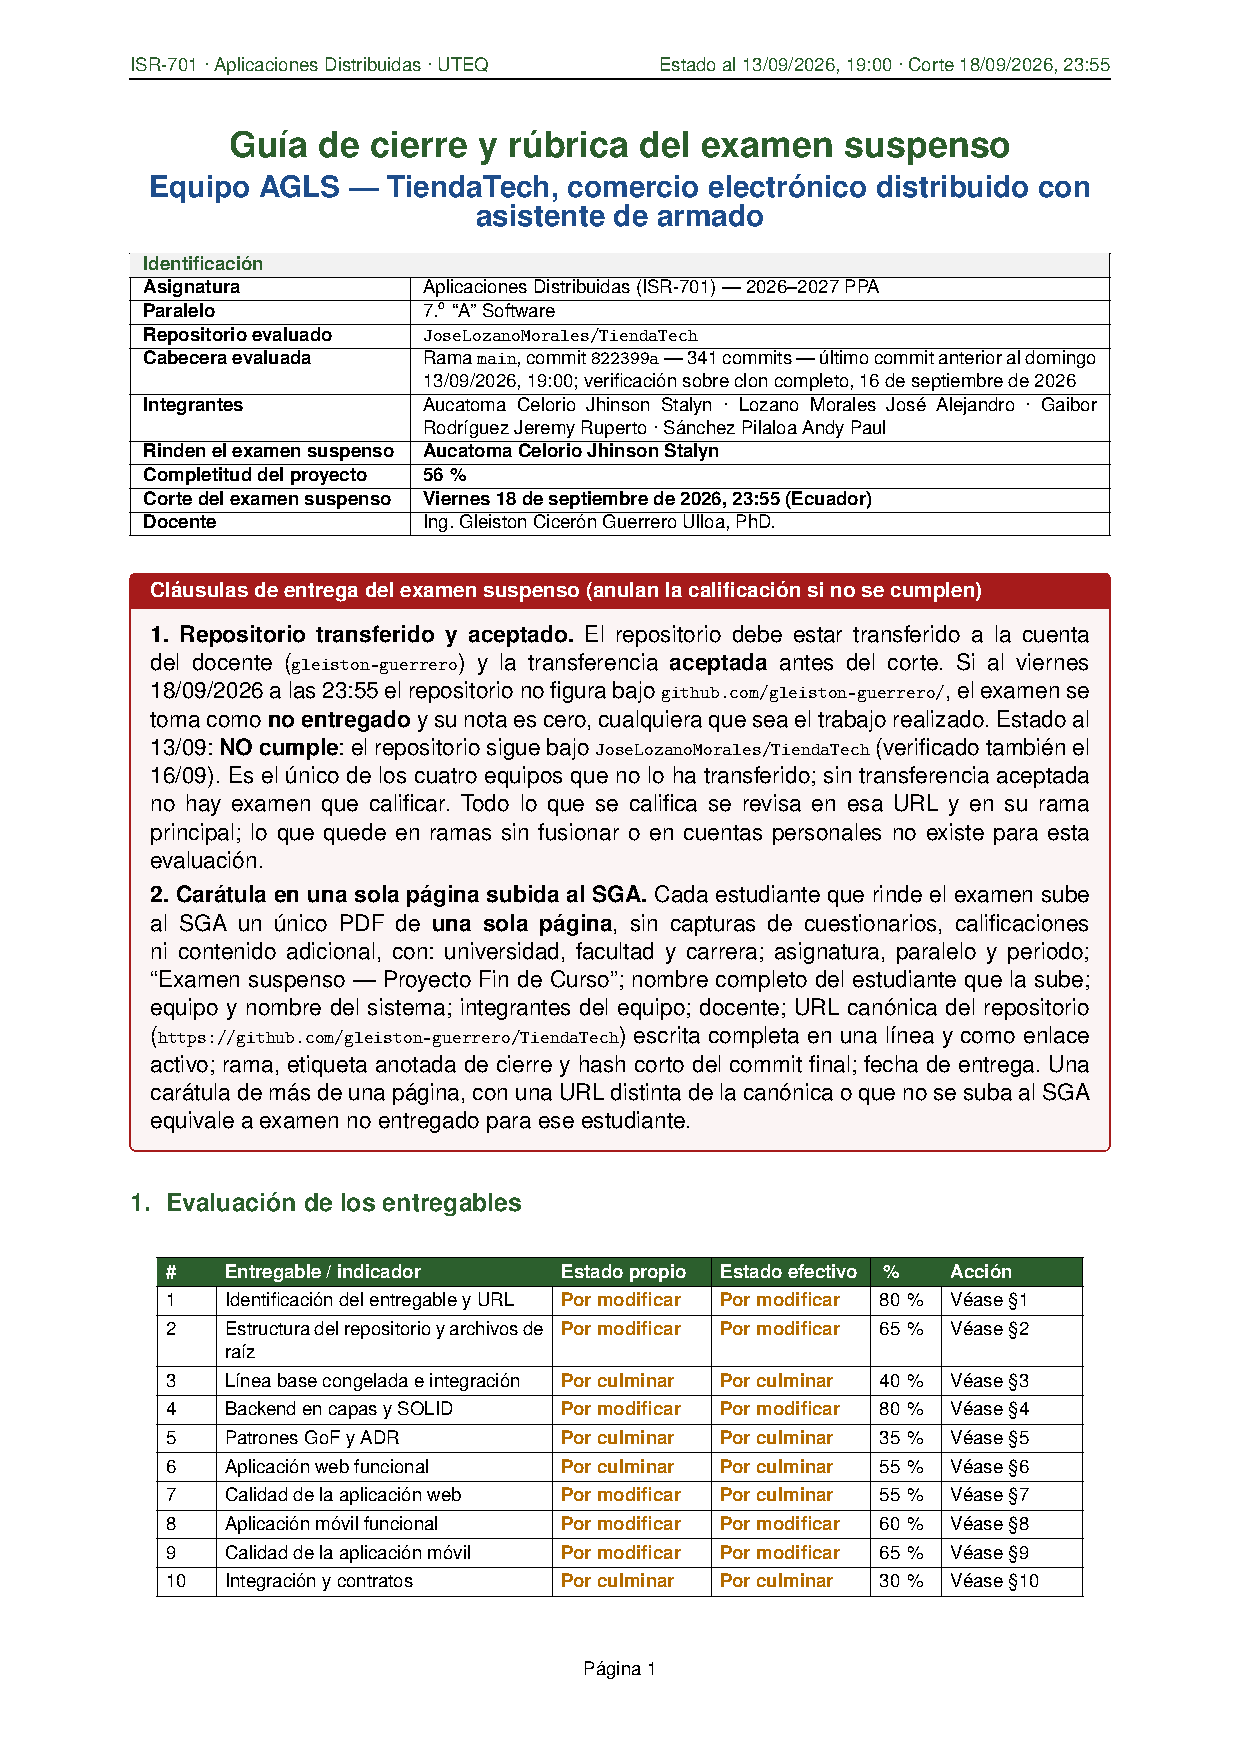
\includepdf[pages=-,addtotoc={1,section,1,AGLS,agls}]{Guia_AGLS.pdf}
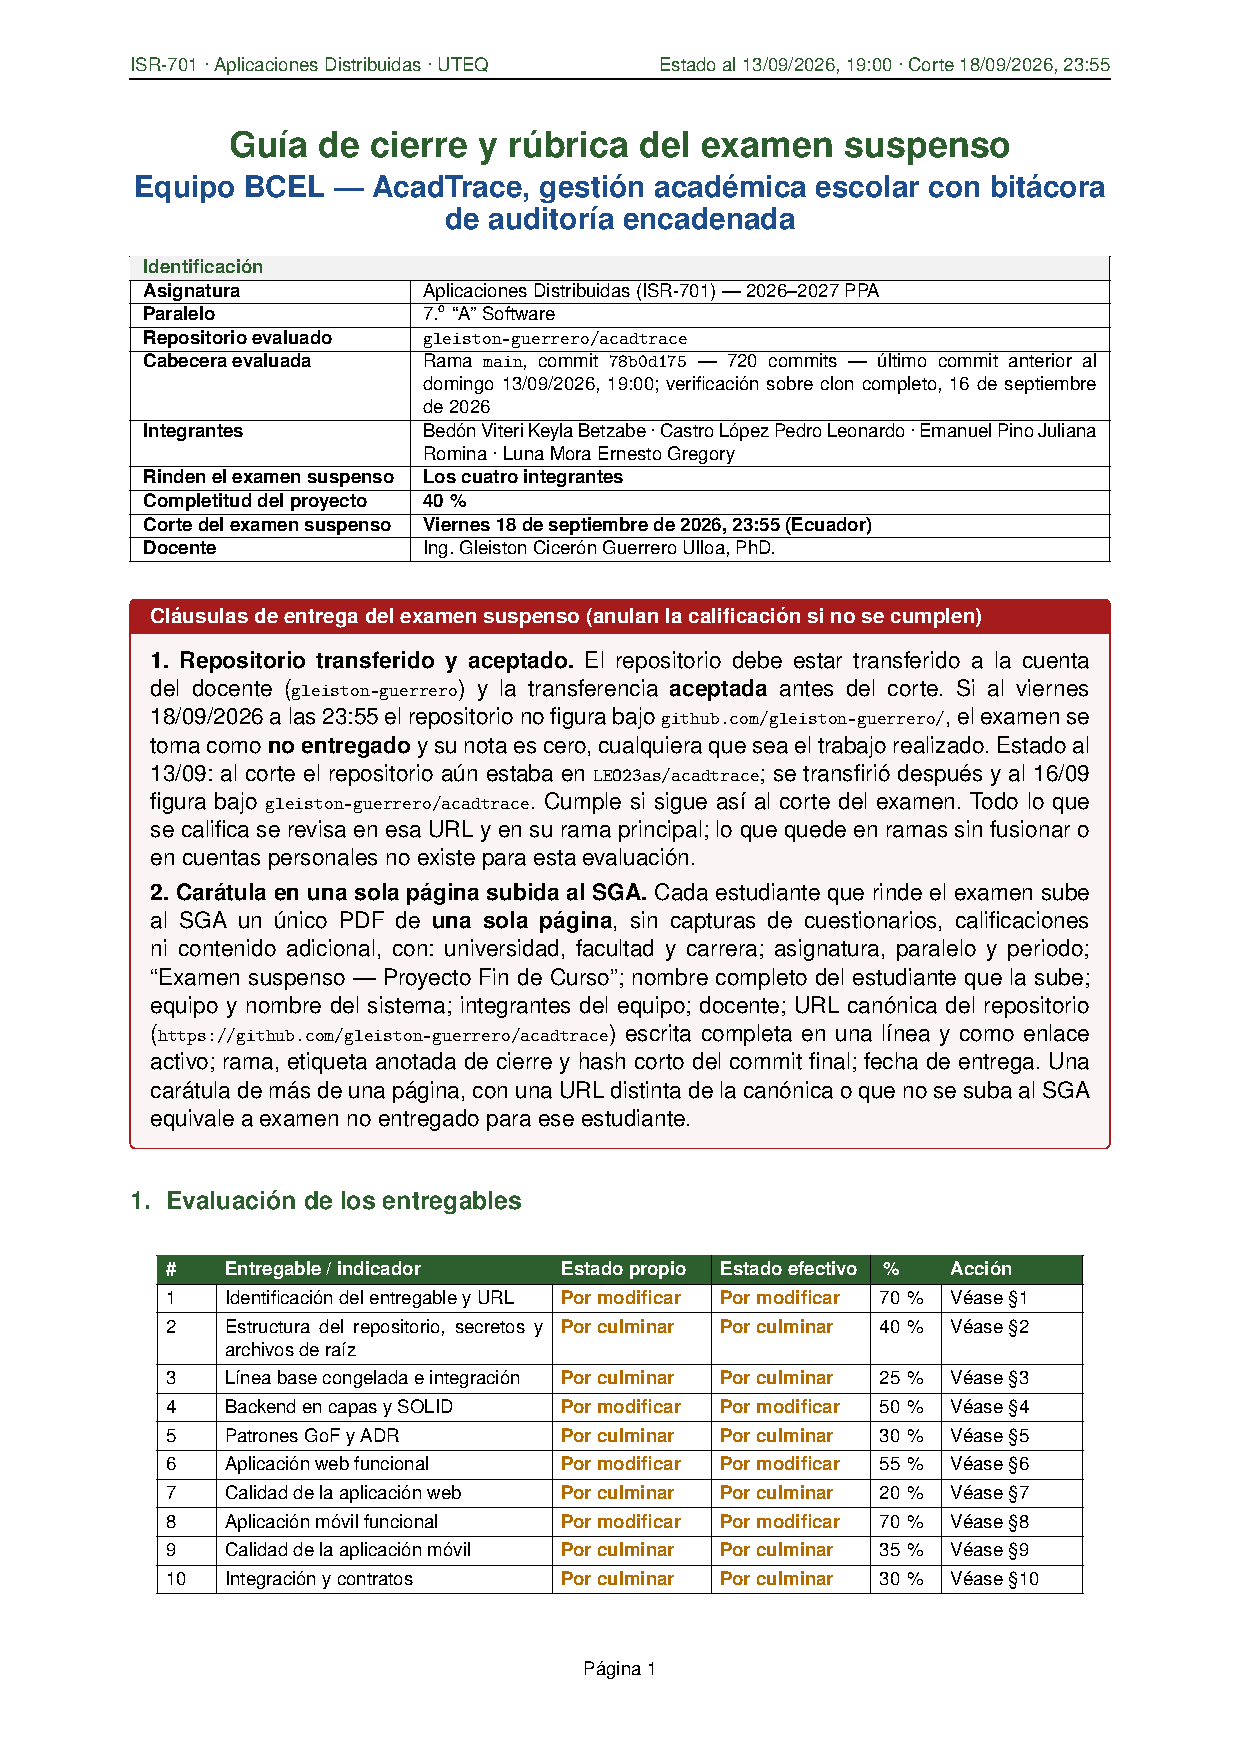
\includepdf[pages=-,addtotoc={1,section,1,BCEL,bcel}]{Guia_BCEL.pdf}
\end{document}
